\iffalse
This file is protected by Copyright. Please refer to the COPYRIGHT file
distributed with this source distribution.

This file is part of OpenCPI <http://www.opencpi.org>

OpenCPI is free software: you can redistribute it and/or modify it under the
terms of the GNU Lesser General Public License as published by the Free Software
Foundation, either version 3 of the License, or (at your option) any later
version.

OpenCPI is distributed in the hope that it will be useful, but WITHOUT ANY
WARRANTY; without even the implied warranty of MERCHANTABILITY or FITNESS FOR A
PARTICULAR PURPOSE. See the GNU Lesser General Public License for more details.

You should have received a copy of the GNU Lesser General Public License along
with this program. If not, see <http://www.gnu.org/licenses/>.
\fi

%----------------------------------------------------------------------------------------
% Update the docTitle and docVersion per document
%----------------------------------------------------------------------------------------
\def\docTitle{OpenCPI\\ FSK App Guide}
\def\docVersion{1.6}
%----------------------------------------------------------------------------------------
\def\snippetpath{../../../../../doc/av/tex/snippets}
% Usage:
% \def\snippetpath{../../../../../doc/av/tex/snippets/}
% % Usage:
% \def\snippetpath{../../../../../doc/av/tex/snippets/}
% % Usage:
% \def\snippetpath{../../../../../doc/av/tex/snippets/}
% \input{\snippetpath/includes}
% From then on, you can use "input" With no paths to get to "snippets"
% You also get all "major" snippets not part of the global LaTeX_Header
% NOTE: If not using the global LaTeX_Header, you need to
% \usepackage{ifthen} to use the \githubio macro

\hyphenation{ANGRY-VIPER} % Tell it where to hyphenate
\hyphenation{Cent-OS} % Tell it where to hyphenate
\hyphenation{install-ation} % Tell it where to hyphenate

\newcommand{\todo}[1]{\textcolor{red}{TODO: #1}\PackageWarning{TODO:}{#1}} % To do notes
\newcommand{\code}[1]{\texttt{#1}} % For inline code snippet or command line
\newcommand{\sref}[1]{Section~\ref{#1}} % To quickly reference a section

% To quickly reference a versioned PDF on github.io
% \def\ocpiversion{1.5.0}
\def\ocpiversion{1.5.0rc4} % TEMPORARY

% This gives a link to github.io document. By default, it puts the filename.
% You can optionally change the link, e.g.
% \githubio{FPGA\_Vendor\_Tools\_Installation\_Guide.pdf} vs.
% \githubio[\textit{FPGA Vendor Tools Installation Guide}]{FPGA\_Vendor\_Tools\_Installation\_Guide.pdf}
% or if you want the raw ugly URL to come out, \githubioURL{FPGA_Vendor_Tools_Installation_Guide.pdf}
\newcommand{\githubio}[2][]{% The default is for FIRST param!
\href{http://opencpi.github.io/releases/\ocpiversion/#2}{\ifthenelse{\equal{#1}{}}{\texttt{#2}}{#1}}}
\newcommand{\githubioURL}[1]{\url{http://opencpi.github.io/releases/\ocpiversion/#1}}

% Fix import paths
\makeatletter
\def\input@path{{\snippetpath/}}
\makeatother

% From then on, you can use "input" With no paths to get to "snippets"
% You also get all "major" snippets not part of the global LaTeX_Header
% NOTE: If not using the global LaTeX_Header, you need to
% \usepackage{ifthen} to use the \githubio macro

\hyphenation{ANGRY-VIPER} % Tell it where to hyphenate
\hyphenation{Cent-OS} % Tell it where to hyphenate
\hyphenation{install-ation} % Tell it where to hyphenate

\newcommand{\todo}[1]{\textcolor{red}{TODO: #1}\PackageWarning{TODO:}{#1}} % To do notes
\newcommand{\code}[1]{\texttt{#1}} % For inline code snippet or command line
\newcommand{\sref}[1]{Section~\ref{#1}} % To quickly reference a section

% To quickly reference a versioned PDF on github.io
% \def\ocpiversion{1.5.0}
\def\ocpiversion{1.5.0rc4} % TEMPORARY

% This gives a link to github.io document. By default, it puts the filename.
% You can optionally change the link, e.g.
% \githubio{FPGA\_Vendor\_Tools\_Installation\_Guide.pdf} vs.
% \githubio[\textit{FPGA Vendor Tools Installation Guide}]{FPGA\_Vendor\_Tools\_Installation\_Guide.pdf}
% or if you want the raw ugly URL to come out, \githubioURL{FPGA_Vendor_Tools_Installation_Guide.pdf}
\newcommand{\githubio}[2][]{% The default is for FIRST param!
\href{http://opencpi.github.io/releases/\ocpiversion/#2}{\ifthenelse{\equal{#1}{}}{\texttt{#2}}{#1}}}
\newcommand{\githubioURL}[1]{\url{http://opencpi.github.io/releases/\ocpiversion/#1}}

% Fix import paths
\makeatletter
\def\input@path{{\snippetpath/}}
\makeatother

% From then on, you can use "input" With no paths to get to "snippets"
% You also get all "major" snippets not part of the global LaTeX_Header
% NOTE: If not using the global LaTeX_Header, you need to
% \usepackage{ifthen} to use the \githubio macro

\hyphenation{ANGRY-VIPER} % Tell it where to hyphenate
\hyphenation{Cent-OS} % Tell it where to hyphenate
\hyphenation{install-ation} % Tell it where to hyphenate

\newcommand{\todo}[1]{\textcolor{red}{TODO: #1}\PackageWarning{TODO:}{#1}} % To do notes
\newcommand{\code}[1]{\texttt{#1}} % For inline code snippet or command line
\newcommand{\sref}[1]{Section~\ref{#1}} % To quickly reference a section

% To quickly reference a versioned PDF on github.io
% \def\ocpiversion{1.5.0}
\def\ocpiversion{1.5.0rc4} % TEMPORARY

% This gives a link to github.io document. By default, it puts the filename.
% You can optionally change the link, e.g.
% \githubio{FPGA\_Vendor\_Tools\_Installation\_Guide.pdf} vs.
% \githubio[\textit{FPGA Vendor Tools Installation Guide}]{FPGA\_Vendor\_Tools\_Installation\_Guide.pdf}
% or if you want the raw ugly URL to come out, \githubioURL{FPGA_Vendor_Tools_Installation_Guide.pdf}
\newcommand{\githubio}[2][]{% The default is for FIRST param!
\href{http://opencpi.github.io/releases/\ocpiversion/#2}{\ifthenelse{\equal{#1}{}}{\texttt{#2}}{#1}}}
\newcommand{\githubioURL}[1]{\url{http://opencpi.github.io/releases/\ocpiversion/#1}}

% Fix import paths
\makeatletter
\def\input@path{{\snippetpath/}}
\makeatother

\documentclass{article}
\iffalse
This file is protected by Copyright. Please refer to the COPYRIGHT file
distributed with this source distribution.

This file is part of OpenCPI <http://www.opencpi.org>

OpenCPI is free software: you can redistribute it and/or modify it under the
terms of the GNU Lesser General Public License as published by the Free Software
Foundation, either version 3 of the License, or (at your option) any later
version.

OpenCPI is distributed in the hope that it will be useful, but WITHOUT ANY
WARRANTY; without even the implied warranty of MERCHANTABILITY or FITNESS FOR A
PARTICULAR PURPOSE. See the GNU Lesser General Public License for more details.

You should have received a copy of the GNU Lesser General Public License along
with this program. If not, see <http://www.gnu.org/licenses/>.
\fi
\author{} % Force author to be blank
%----------------------------------------------------------------------------------------
% Paper size, orientation and margins
%----------------------------------------------------------------------------------------
\usepackage{geometry}
\geometry{
        letterpaper, % paper type
        portrait,    % text direction
        left=.75in,  % left margin
        top=.75in,   % top margin
        right=.75in, % right margin
        bottom=.75in % bottom margin
 }
%----------------------------------------------------------------------------------------
% Header/Footer
%----------------------------------------------------------------------------------------
\usepackage{fancyhdr} \pagestyle{fancy} % required for fancy headers
\renewcommand{\headrulewidth}{0.5pt}
\renewcommand{\footrulewidth}{0.5pt}
\rhead{\small{ANGRYVIPER Team}}
% \rfoot{\thepage}
%----------------------------------------------------------------------------------------
% Appendix packages
%----------------------------------------------------------------------------------------
\usepackage[toc,page]{appendix}
%----------------------------------------------------------------------------------------
% Defined Commands & Renamed Commands
%----------------------------------------------------------------------------------------
\renewcommand{\contentsname}{Table of Contents}
\renewcommand{\listfigurename}{List of Figures}
\renewcommand{\listtablename}{List of Tables}
%----------------------------------------------------------------------------------------
% Various packages
%----------------------------------------------------------------------------------------
\usepackage[usenames,dvipsnames]{xcolor} % for color names see https://en.wikibooks.org/wiki/LaTeX/Colors
\usepackage{hyperref}  % for linking urls and lists
\usepackage{graphicx}  % for including pictures by file
\usepackage{listings}  % for coding language styles
\usepackage{rotating}  % for sideways table
\usepackage{pifont}    % for sideways table
\usepackage{pdflscape} % for landscape view
\usepackage{subfig}
\usepackage{xstring}
\uchyph=0 % Never hyphenate acronyms like RCC (I think this overrides ANGRYVIPER above)
\renewcommand\_{\textunderscore\allowbreak} % Allow words to break/newline on underscores
%----------------------------------------------------------------------------------------
% Table packages
%----------------------------------------------------------------------------------------
\usepackage{longtable} % for long possibly multi-page tables
\usepackage{tabularx} % c=center,l=left,r=right,X=fill
% These define tabularx columns "C" and "R" to match "X" but center/right aligned
\newcolumntype{C}{>{\centering\arraybackslash}X}
\newcolumntype{R}{>{\raggedleft\arraybackslash}X}
\usepackage{float}
\floatstyle{plaintop}
\usepackage[tableposition=top]{caption}
\newcolumntype{P}[1]{>{\centering\arraybackslash}p{#1}}
\newcolumntype{M}[1]{>{\centering\arraybackslash}m{#1}}
%----------------------------------------------------------------------------------------
% Block Diagram / FSM Drawings
%----------------------------------------------------------------------------------------
\usepackage{tikz}
\usetikzlibrary{shapes,arrows,fit,positioning}
\usetikzlibrary{automata} % used for the fsm
%----------------------------------------------------------------------------------------
% Colors Used
%----------------------------------------------------------------------------------------
\usepackage{colortbl}
\definecolor{blue}{rgb}{.7,.8,.9}
\definecolor{ceruleanblue}{rgb}{0.16, 0.32, 0.75}
\definecolor{drkgreen}{rgb}{0,0.6,0}
\definecolor{deepmagenta}{rgb}{0.8, 0.0, 0.8}
\definecolor{cyan}{rgb}{0.0,0.6,0.6}
\definecolor{maroon}{rgb}{0.5,0,0}
%----------------------------------------------------------------------------------------
% VHDL Coding Language Style
% modified from: http://latex-community.org/forum/viewtopic.php?f=44&t=22076
%----------------------------------------------------------------------------------------
\lstdefinelanguage{VHDL}
{
        basicstyle=\ttfamily\footnotesize,
        columns=fullflexible,keepspaces,      % https://tex.stackexchange.com/a/46695/87531
        keywordstyle=\color{ceruleanblue},
        commentstyle=\color{drkgreen},
        morekeywords={
    library,use,all,entity,is,port,in,out,end,architecture,of,
    begin,and, signal, when, if, else, process, end,
        },
        morecomment=[l]--
}
%----------------------------------------------------------------------------------------
% XML Coding Language Style
% modified from: http://tex.stackexchange.com/questions/10255/xml-syntax-highlighting
%----------------------------------------------------------------------------------------
\lstdefinelanguage{XML}
{
        basicstyle=\ttfamily\footnotesize,
        columns=fullflexible,keepspaces,
        morestring=[s]{"}{"},
        morecomment=[s]{!--}{--},
        commentstyle=\color{drkgreen},
        moredelim=[s][\color{black}]{>}{<},
        moredelim=[s][\color{cyan}]{\ }{=},
        stringstyle=\color{maroon},
        identifierstyle=\color{ceruleanblue}
}
%----------------------------------------------------------------------------------------
% DIFF Coding Language Style
% modified from http://tex.stackexchange.com/questions/50176/highlighting-a-diff-file
%----------------------------------------------------------------------------------------
\lstdefinelanguage{diff}
{
        basicstyle=\ttfamily\footnotesize,
        columns=fullflexible,keepspaces,
        breaklines=true,                                % wrap text
        morecomment=[f][\color{ceruleanblue}]{@@},      % group identifier
        morecomment=[f][\color{red}]-,                  % deleted lines
        morecomment=[f][\color{drkgreen}]+,             % added lines
        morecomment=[f][\color{deepmagenta}]{---},      % Diff header lines (must appear after +,-)
        morecomment=[f][\color{deepmagenta}]{+++},
}
%----------------------------------------------------------------------------------------
% Python Coding Language Style
% modified from
%----------------------------------------------------------------------------------------
\lstdefinelanguage{python}
{
        basicstyle=\ttfamily\footnotesize,
        columns=fullflexible,keepspaces,
        keywordstyle=\color{ceruleanblue},
        commentstyle=\color{drkgreen},
        stringstyle=\color{orange},
        morekeywords={
    print, if, sys, len, from, import, as, open,close, def, main, for, else, write, read, range,
        },
        comment=[l]{\#}
}
%----------------------------------------------------------------------------------------
% Fontsize Notes in order from smallest to largest
%----------------------------------------------------------------------------------------
%    \tiny
%    \scriptsize
%    \footnotesize
%    \small
%    \normalsize
%    \large
%    \Large
%    \LARGE
%    \huge
%    \Huge

\setlength\parindent{0pt}
\date{Version \docVersion} % Force date to be blank and override date with version
\title{\docTitle}
\lhead{FSK App Guide}
%----------------------------------------------------------------------------------------
%\usepackage[T1]{fontenc} % http://tex.stackexchange.com/a/181119
\usepackage{graphicx}
\graphicspath{ {figures/} }
\usepackage{textcomp}
\usepackage{amsmath}

\begin{document}
\maketitle
%\thispagestyle{fancy}
\newpage
	\begin{center}
	\textit{\textbf{Revision History}}
		\begin{table}[H]
		\label{table:revisions} % Add "[H]" to force placement of table
			\begin{tabularx}{\textwidth}{|c|X|l|}
			\hline
			\rowcolor{blue}
			\textbf{Revision} & \textbf{Description of Change} & \textbf{Date} \\
		    \hline
		    v1.1 & Initial Release & 3/2017 \\
		    \hline
		    v1.2 & Updated for OpenCPI Release 1.2 & 8/2017 \\
			\hline
			v1.3 & Updated for OpenCPI Release 1.3 & 1/2018 \\
			\hline
			v1.3.1 & Updated for OpenCPI Release 1.3.1, including FMCOMMS2/3 support & 3/2018 \\
			\hline
			v1.4 & Updated recommendations for configuring \path{OCPI_LIBRARY_PATH} & 9/2018 \\
			\hline
			v1.5 & Deprecated Zipper; Moved to Appendix & 3/2019 \\
			\hline
			v1.6 & Added RCC only FSK Application mode & 8/2019 \\
			\hline
			\end{tabularx}
		\end{table}
	\end{center}

\newpage
\tableofcontents
\pagebreak
\section{Document Scope}
This document describes the OpenCPI Frequency Shift Keying Modulation (FSK) demo application. It includes a description of the application, instructions to setup the hardware, build of bitstreams, and execution of the application itself on various platforms.

\section{Supported Setups}
This app is supported various hardware software setups.
\subsection{Supported Hardware Setups}
This app is supported on the following hardware configurations:
\begin{itemize}
  \item Zedboard/FMCOMMS2
  \item Zedboard/FMCOMMS3
  \item x86/ML605/FMCOMMS2 in FMC LPC slot
  \item x86/ML605/FMCOMMS3 in FMC LPC slot
  \item Matchstiq-Z1
\end{itemize}

\subsection{Supported Hardware Setups}
This app can run without any hardware in software using RCC-only mode.
\newpage % This is needed or the figures split weird; each mode with a picture gets a page I guess
\section{Application Modes}
The FSK App may be run in one of six available modes: \textit{filerw\_rcc}, \textit{filerw}, \textit{rx}, \textit{tx}, \textit{txrx}, and  \textit{bbloopback}.
\subsection{filerw\_rcc mode}
The \textit{filerw\_rcc} mode uses only RCC application workers and implements a simplified version\footnote{The \textit{CIC Interpolator} and \textit{CIC Decimator} were removed because their function isn't required when not transmitting over-the-air and RCC versions would not provide the throughput required.} of the full FSK App.
This application allows testing the OpenCPI framework on an RCC platform without depending on any HDL code.
A block diagram of the FSK App \textit{filerw\_rcc} mode can be seen in Figure \ref{fig:filerw_rcc_mode_block_diagram}.
% TODO: These could be vector-based TeX native?
\newcommand{\FSKAppModeFigure}[2]{
\begin{figure}[H]
  \centering
  \includegraphics[scale=.55]{#2}
  \caption{FSK App \textit{#1} mode Block Diagram}
  \label{fig:#2}
\end{figure}
}
\FSKAppModeFigure{filerw\_rcc}{filerw_rcc_mode_block_diagram}
\newpage\subsection{filerw mode}
The \textit{filerw} mode uses file\_read and file\_write workers to process the input using only application workers (platform agnostic) in a purely digital fashion.
A block diagram of the FSK App \textit{filerw} mode can be seen in Figure \ref{fig:filerw_mode_block_diagram}.
\FSKAppModeFigure{filerw}{filerw_mode_block_diagram}

\newpage\subsection{rx mode}
The \textit{rx} mode inputs I+Q data from the ADC and processes the FSK signal down to bits that are written to file.
A block diagram of the FSK App \textit{rx} mode can be seen in Figure \ref{fig:rx_mode_block_diagram}.
The \textit{rx} mode requires a second radio operating in \textit{tx} mode to provide the data signal.
\FSKAppModeFigure{rx}{rx_mode_block_diagram}

\newpage\subsection{tx mode}
The \textit{tx} mode inputs a file from disk, modulates the input as a FSK signal, and transmits the input via the DAC.
A block diagram of the FSK App \textit{tx} mode can be seen in Figure \ref{fig:tx_mode_block_diagram}.
The \textit{tx} mode requires a second radio operating in \textit{rx} mode to receive and verify the signal.
\FSKAppModeFigure{tx}{tx_mode_block_diagram}

\newpage\subsection{txrx mode}
The \textit{txrx} mode is the full transceiver mode of the application which combines the functionality of Figures \ref{fig:rx_mode_block_diagram} and \ref{fig:tx_mode_block_diagram} into a single application.
This mode transmits input file data as the radio RF TX output and inputs RF RX radio input that is written to file.
%\newpage
\subsection{bbloopback mode}
The \textit{bbloopback} mode utilizes the same HDL assembly and application XML as the \textit{txrx} mode, but sets a built-in test mode of the transceiver to loopback analog data at baseband.\par\medskip
% This is here to direct people who ask about GPIO workers in the future
\subsection{Controlling output pins using matchstiq\_z1\_gp\_out worker}
This section doesn't directly apply to the FSK App, but is given as an example of controlling general purpose output pins on the matchstiq\_z1.
The \textit{tx}, \textit{txrx}, and \textit{bbloopback} modes for the Matchstiq-Z1 contain the matchstiq\_z1\_gp\_out device worker which can control the three GPIO pins present on the Matchstiq-Z1.
These applications\footnote{The application XMLs can be examined to learn how to use the device worker.} are a working example of the matchstiq\_z1\_gp\_out device worker controlling GPIO pins.
See the matchstiq\_z1\_gp\_out datasheet for more info.
%\par\medskip


\subsection{Application Specifications}
\subsubsection{Baud Rate}
The baud rate for the application is based on the following properties:
	\begin{itemize}
		\item ADC/DAC Sample Rate (S)
		\item CIC Decimation/Interpolation Factor (R)
		\item Number of zeros inserted between symbols (Z)
	\end{itemize}
It can be computed using the following equation:
	      \begin{equation}
	      	Baud\ Rate = S\ /\ R\ /\ (Z +1)
	      \end{equation}
Using the default settings for the Matchstiq Z1 platform, the resulting baud rate is 64 kbaud.
	      \begin{equation}
	      	Baud\ Rate = S\ /\ R\ /\ (Z+1) = 39,936,000 \ /\ 16\ /\ (38+1) \ =\ 64000
	      \end{equation}
\subsubsection{Frequency Deviation}
The theoretical FSK frequency deviation is calculated as follows. The bits of the input file are converted to Q0.15 symbols by the mfsk\_mapper worker, where the symbol values are determined by the value of the worker's symbols property, which is an array. The following equation corresponds to the values mapped from bits, with $s$ representing the bit value. Note that division by $2^{15}$ accounts for the Q0.15 value interpretation. The mfsk\_mapper worker's symbols array property value is fixed to the values $symbols[0]=-32768$ and $symbols[1]=32767$ in all OASs used by the ACI.
	\begin{equation} \label{eq:map_out_val}
		x_{mfsk\_mapper,out,s}=\frac{symbols[s]}{2^{15}},
    s \in [0..1] % https://en.wikipedia.org/wiki/Interval_(mathematics)#Integer_intervals
	\end{equation}
The value of these symbols is unmodified as they pass through the zero\_pad worker.
	\begin{equation} \label{eq:zp_out_val}
		x_{zero\_pad\_mapper,out,s}=x_{mfsk\_mapper,out,s}
	\end{equation}
The zero-padded symbols then pass through the fir\_real\_see worker whose taps are read from a file at runtime. The gen\_rrcos\_taps.py script runs at application buildtime to generate the tap file for a root-raised-cosine filter. The application \path{Makefile} passes an argument to the script that forces the filter taps to be scaled such that the maximum tap value amplitude $maxTap$ is 4096, which corresponds to the Q0.15 value $4096/2^{15}=0.125$. Because root-raised-cosine filters do not obey the Nyquist ISI criterion, the incoming symbol values will undergo an amplitude adjustment that will vary per symbol, as shown in Figure \ref{fig:tx_fir_data}. In order to to proceed with frequency deviation calculation, the nominal symbol values are approximated as being multiplied by the maximum Q0.15 tap value while passing through the fir\_real\_sse worker.
	\begin{figure}[ht]
	 	\centering
	 	\begin{minipage}{0.7\textwidth}
			\centering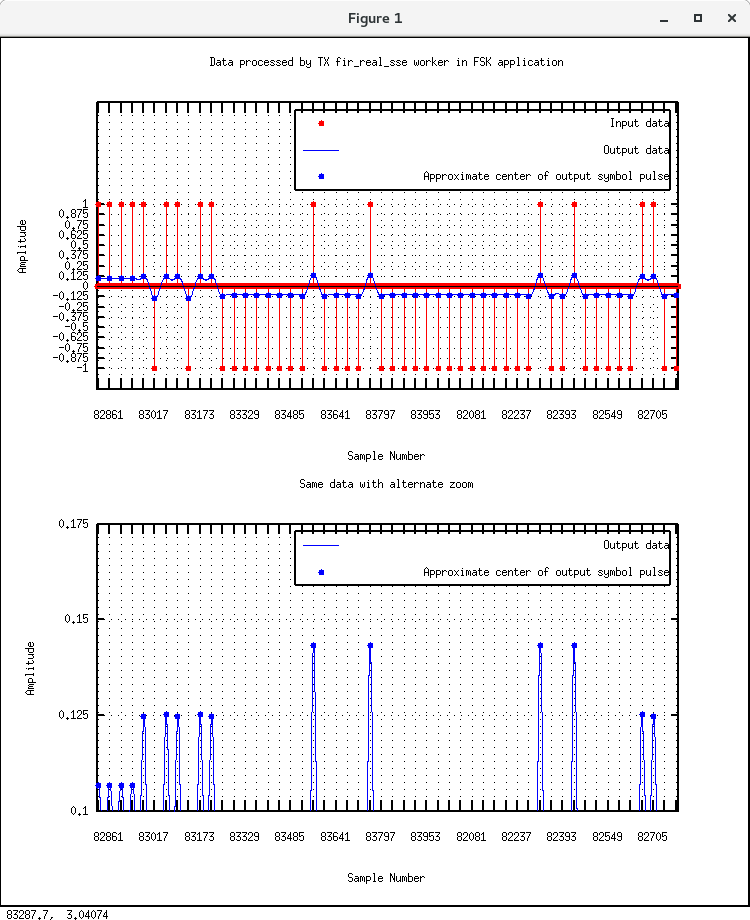
\includegraphics[trim=0.5cm 1cm 1cm 1.5cm,clip,width=1.0\linewidth]{fir_real_sse_data}
			\caption{Data processed by TX fir\_real\_sse worker.}
			\label{fig:tx_fir_data}
		\end{minipage}
	\end{figure}

	\begin{equation} \label{eq:fir_out_val}
		x_{fir\_real\_sse,out,s,nom} = \frac{maxTap}{2^{15}} * x_{zero\_pad\_mapper,out,s}
	\end{equation}
The frequency modulation performed by the phase\_to\_amp\_cordic worker assigns frequency according to the following formula. Note that $x_{fir\_real\_sse,out}$ is in the Q0.15 format.

	\begin{equation}
		f_{phase\_to\_amp\_cordic,out} = \pi * x_{fir\_real\_sse,out} \ \frac{\text{radians}}{\text{sample}}
	\end{equation}
The nominal space/mark frequencies at the output of the phase\_to\_amp\_cordic worker is given as:
	\begin{equation}
		f_{phase\_to\_amp\_cordic,out,s,nom} = \pi * \frac{maxTap}{2^{15}} * \frac{symbols[s]}{2^{15}} \ \frac{\text{radians}}{\text{sample}}
	\end{equation}
Figure \ref{fig:mark_space_freq} displays the nominal space and mark frequencies versus that actual instantaneous frequency of the output of the phase\_to\_amp\_cordic worker that will occur at runtime.
	\begin{figure}[ht]
	 	\centering
	 	\begin{minipage}{0.7\textwidth}
			\centering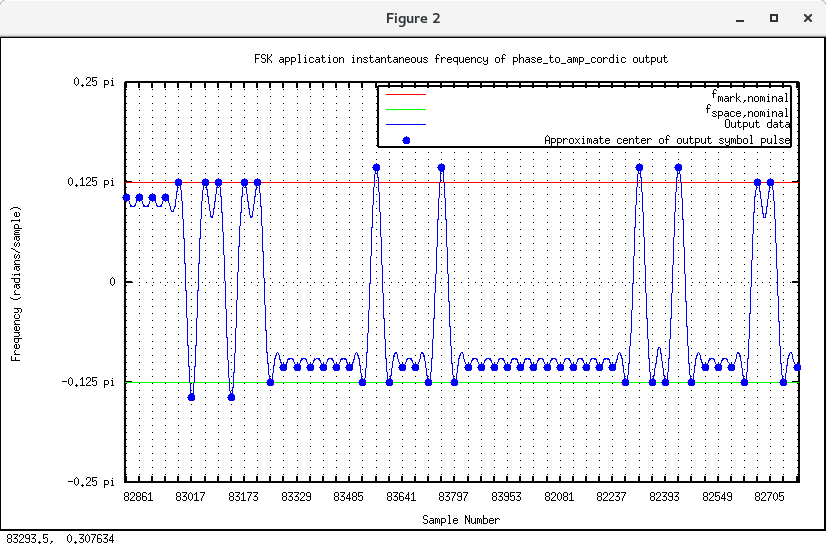
\includegraphics[trim=0.2cm 0.6cm 0.1cm 2.8cm,clip,width=1.0\linewidth]{mark_space_freq}
			\caption{Instantaneous frequency of phase\_to\_amp\_cordic output.}
			\label{fig:mark_space_freq}
		\end{minipage}
	\end{figure}
The output of phase\_to\_amp\_cordic is upsampled by an interpolating CIC filter, which has the effect of dividing the space/mark frequencies. The interpolation factor is fixed via the parameter property/value of $R=16$ within all assemblies used by the ACI and all its OASs.
	\begin{equation} \label{eq:cic}
		f_{cic\_int,out,s,nom} = \frac{f_{phase\_to\_amp\_cordic,out,s,nom}}{R}
	\end{equation}
The output data of the CIC is passed to the DAC, which has a configurable sample rate $f_s$. The resulting space/mark frequencies at the output of the DAC is given as:
	\begin{equation} \label{eq:output_freq_0}
		f_{DAC,out,s,nominal} = \Bigg[ f_{cic\_int,out,s,nom} \frac{radians}{sample} \Bigg] * \Bigg[ fs \frac{samples}{second} \Bigg] * \Bigg[ \frac{1}{2\pi \ radians} \Bigg] = \frac{maxTap}{2^{15}} * \frac{symbols[s]}{2^{16}} * \frac{f_s}{R} \ \text{Hz}
	\end{equation}
This results in a final frequency deviation calculation:
	\begin{align*} \label{eq:freq_deviation}
		f_{\Delta,nominal} &= f_{DAC,out,1,nominal} - f_{DAC,out,0,nominal}
		= \frac{maxTap}{2^{15}} * \frac{symbols[1]-symbols[0]}{2^{16}} * \frac{f_s}{R} \\
		&= 0.125 * \frac{32767 - (-32768)}{2^{16}} * \frac{f_s}{16}
		= \frac{65535}{2^{23}} f_s \ \text{Hz}
	\end{align*}
Using the ACI's default prompted setting of $f_s=4,000,000$ Hz for the FMCOMMS2/3 transceivers, the resulting nominal frequency deviation would be approximately 31,249.5 Hz.

\newpage
\section{Building the Application}
\subsection{Dependencies}
The tables below breakdown the workers used within the various platforms and modes of the FSK App. Additionally, Appendix~\ref{app:Worker_Parameters} shows the exact worker configurations used in the HDL assemblies. See the individual component data sheets for more information and build instructions. Similarly, the HDL platform worker and configurations for the intended radio must be compiled prior to building the various FSK bitstreams.
\subsection{FSK Mode Configurations}
	% Make new row command - single space is unchecked; anything else checks (7 columns wide)
	\newcommand{\checkrow}[7]{{#1} &
		\ifthenelse{ \equal{#2}{ } }{}{\ding{51}} &
		\ifthenelse{ \equal{#3}{ } }{}{\ding{51}} &
		\ifthenelse{ \equal{#4}{ } }{}{\ding{51}} &
		\ifthenelse{ \equal{#5}{ } }{}{\ding{51}} &
		\ifthenelse{ \equal{#6}{ } }{}{\ding{51}} &
		\ifthenelse{ \equal{#7}{ } }{}{\ding{51}}\\ \hline}
\subsubsection{Common to all Hardware}
	\begin{tabular}{|c|c|c|c|c|c|c|}
	\hline
	\rowcolor{blue}
	Application XML & filerw & filerw\_rcc & rx & tx & txrx & bbloopback \\
	\hline
	\checkrow{app\_fsk\_filerw (dependency only, no build required)}{x}{ }{ }{ }{ }{ }
	\checkrow{app\_fsk\_filerw\_rcc (dependency only, no build required)}{ }{x}{ }{ }{ }{ }
	\rowcolor{blue}
	HDL Assemblies & filerw & filerw\_rcc & rx & tx & txrx & bbloopback \\
	\hline
	\checkrow{fsk\_filerw}{x}{ }{ }{ }{ }{ }
	\checkrow{dc\_offset\_iq\_imbalance\_mixer\_cic\_dec\_rp\_cordic\_fir\_real}{ }{ }{x}{ }{ }{ }
	\checkrow{mfsk2\_zp16\_fir\_real\_phase\_to\_amp\_cordic\_cic\_int}{ }{ }{ }{x}{ }{ }
	\checkrow{fsk\_modem}{ }{ }{ }{ }{x}{x}
	\rowcolor{blue}
	RX Path Workers & filerw & filerw\_rcc & rx & tx & txrx & bbloopback \\
	\hline
	\checkrow{dc\_offset\_filter.hdl}{ }{ }{x}{ }{x}{x}
	\checkrow{iq\_imbalance\_fixer.hdl}{ }{ }{x}{ }{x}{x}
	\checkrow{complex\_mixer.hdl}{x}{ }{x}{ }{x}{x}
	\checkrow{cic\_dec.hdl}{x}{ }{x}{ }{x}{x}
	\checkrow{rp\_cordic.hdl}{x}{ }{x}{ }{x}{x}
	\checkrow{rp\_cordic\_for\_fskapp.rcc}{ }{x}{ }{ }{ }{ }
	\checkrow{fir\_real\_sse.hdl}{x}{ }{x}{ }{x}{x}
	\checkrow{fir\_real\_sse\_for\_fskapp.rcc}{ }{x}{ }{ }{ }{ }
	\checkrow{baudTracking.rcc}{x}{x}{x}{ }{x}{x}
	\checkrow{real\_digitizer.rcc}{x}{x}{x}{ }{x}{x}
	\checkrow{file\_write.rcc}{x}{x}{x}{ }{x}{x}
	\rowcolor{blue}
	TX Path Workers & filerw & filerw\_rcc & rx & tx & txrx & bbloopback \\
	\hline
	\checkrow{file\_read.rcc}{x}{x}{ }{x}{x}{x}
	\checkrow{mfsk\_mapper.hdl}{x}{ }{ }{x}{x}{x}
	\checkrow{mfsk\_mapper.rcc}{ }{x}{ }{ }{ }{ }
	\checkrow{zero\_pad.hdl}{x}{ }{ }{x}{x}{x}
	\checkrow{zero\_pad.rcc}{ }{x}{ }{ }{ }{ }
	\checkrow{fir\_real\_sse.hdl}{x}{ }{ }{x}{x}{x}
	\checkrow{fir\_real\_sse\_for\_fskapp.rcc}{ }{x}{ }{ }{ }{ }
	\checkrow{phase\_to\_amp\_cordic.hdl}{x}{ }{ }{x}{x}{x}
	\checkrow{phase\_to\_amp\_cordic.rcc}{ }{x}{ }{ }{ }{ }
	\checkrow{cic\_int.hdl}{x}{ }{ }{x}{x}{x}
	\end{tabular}

\subsubsection{Additional Dependencies for FMCOMMS2}
	% Make new row command - single space is unchecked; anything else checks (6 columns wide)
	\renewcommand{\checkrow}[6]{{#1} &
		\ifthenelse{ \equal{#2}{ } }{}{\ding{51}} &
		\ifthenelse{ \equal{#3}{ } }{}{\ding{51}} &
		\ifthenelse{ \equal{#4}{ } }{}{\ding{51}} &
		\ifthenelse{ \equal{#5}{ } }{}{\ding{51}} &
		\ifthenelse{ \equal{#6}{ } }{}{\ding{51}}\\ \hline}
	\begin{tabular}{|c|c|c|c|c|c|}
	\hline
	\rowcolor{blue}
	Application XML & filerw & rx & tx & txrx & bbloopback \\
	\hline
	\checkrow{app\_fsk\_rx\_fmcomms2 (dependency only, no build required)}{ }{x}{ }{ }{ }
	\checkrow{app\_fsk\_tx\_fmcomms2 (dependency only, no build required)}{ }{ }{x}{ }{ }
	\checkrow{app\_fsk\_txrx\_fmcomms2 (dependency only, no build required)}{ }{ }{ }{x}{ }
	\rowcolor{blue}
	RX or TX Path Workers & filerw & rx & tx & txrx & bbloopback \\
	\hline
	\checkrow{ad9361\_data\_sub.hdl}{ }{x}{x}{x}{ }
	\rowcolor{blue}
	RX Path Workers & filerw & rx & tx & txrx & bbloopback \\
	\checkrow{ad9361\_adc.hdl}{ }{x}{ }{x}{ }
	\checkrow{ad9361\_adc\_sub.hdl}{ }{x}{ }{x}{ }
	\rowcolor{blue}
	TX Path Workers & filerw & rx & tx & txrx & bbloopback \\
	\checkrow{ad9361\_dac.hdl}{ }{ }{x}{x}{ }
	\checkrow{ad9361\_dac\_sub.hdl}{ }{ }{x}{x}{ }
	\rowcolor{blue}
	Endpoint Proxies & filerw & rx & tx & txrx & bbloopback \\
	\checkrow{fmcomms\_2\_3\_rx.rcc}{ }{x}{ }{x}{ }
	\checkrow{fmcomms\_2\_3\_tx.rcc}{ }{ }{x}{x}{ }
	\rowcolor{blue}
	SPI Command and Control & filerw & rx & tx & txrx & bbloopback \\
	\checkrow{ad9361\_config.hdl}{ }{x}{x}{x}{ }
	\checkrow{ad9361\_config\_proxy.rcc}{ }{x}{x}{x}{ }
	\checkrow{ad9361\_spi.hdl}{ }{x}{x}{x}{ }
	\rowcolor{blue}
	I2C Command and Control & filerw & rx & tx & txrx & bbloopback \\
	\hline
	\checkrow{fmcomms\_2\_3\_i2c.hdl}{ }{x}{x}{x}{ }
	\hline
	\end{tabular}

\subsubsection{Additional Dependencies for FMCOMMS3}
	\begin{tabular}{|c|c|c|c|c|c|}
	\hline
	\rowcolor{blue}
	Application XML & filerw & rx & tx & txrx & bbloopback \\
	\hline
	\checkrow{app\_fsk\_rx\_fmcomms3 (dependency only, no build required)}{ }{x}{ }{ }{ }
	\hline
	\checkrow{app\_fsk\_tx\_fmcomms3 (dependency only, no build required)}{ }{ }{x}{ }{ }
	\hline
	\checkrow{app\_fsk\_txrx\_fmcomms3 (dependency only, no build required)}{ }{ }{ }{x}{ }
	\hline
	\rowcolor{blue}
	RX or TX Path Workers & filerw & rx & tx & txrx & bbloopback \\
	\hline
	\checkrow{ad9361\_data\_sub.hdl}{ }{x}{x}{x}{ }
	\rowcolor{blue}
	RX Path Workers & filerw & rx & tx & txrx & bbloopback \\
	\hline
	\checkrow{ad9361\_adc.hdl}{ }{x}{ }{x}{ }
	\hline
	\checkrow{ad9361\_adc\_sub.hdl}{ }{x}{ }{x}{ }
	\hline
	\rowcolor{blue}
	TX Path Workers & filerw & rx & tx & txrx & bbloopback \\
	\hline
	\checkrow{ad9361\_dac.hdl}{ }{ }{x}{x}{ }
	\hline
	\checkrow{ad9361\_dac\_sub.hdl}{ }{ }{x}{x}{ }
	\rowcolor{blue}
	Endpoint Proxies & filerw & rx & tx & txrx & bbloopback \\
	\hline
	\checkrow{fmcomms\_2\_3\_rx.rcc}{ }{x}{ }{x}{ }
	\hline
	\checkrow{fmcomms\_2\_3\_tx.rcc}{ }{ }{x}{x}{ }
	\hline
	\rowcolor{blue}
	SPI Command and Control & filerw & rx & tx & txrx & bbloopback \\
	\hline
	\checkrow{ad9361\_config.hdl}{ }{x}{x}{x}{ }
	\hline
	\checkrow{ad9361\_config\_proxy.rcc}{ }{x}{x}{x}{ }
	\hline
	\checkrow{ad9361\_spi.hdl}{ }{x}{x}{x}{}
	\hline
	\rowcolor{blue}
	I2C Command and Control & filerw & rx & tx & txrx & bbloopback \\
	\hline
	\checkrow{fmcomms\_2\_3\_i2c.hdl}{ }{x}{x}{x}{}
	\hline
	\end{tabular}

\subsubsection{Additional Dependencies for Matchstiq-Z1}
	\begin{tabular}{|c|c|c|c|c|c|}
	\hline
	\rowcolor{blue}
	Application XML & filerw & rx & tx & txrx & bbloopback \\
	\hline
	\checkrow{app\_fsk\_rx\_matchstiq\_z1 (dependency only, no build required)}{ }{x}{ }{ }{ }
	\hline
	\checkrow{app\_fsk\_tx\_matchstiq\_z1 (dependency only, no build required)}{ }{ }{x}{ }{ }
	\hline
	\checkrow{app\_fsk\_txrx\_matchstiq\_z1 (dependency only, no build required)}{ }{ }{ }{x}{x}
	\hline
	\rowcolor{blue}
	RX Path Workers & filerw & rx & tx & txrx & bbloopback \\
	\hline
	\checkrow{lime\_adc.hdl}{ }{x}{ }{x}{x}
	\hline
	\rowcolor{blue}
	TX Path Workers & filerw & rx & tx & txrx & bbloopback \\
	\hline
	\checkrow{lime\_dac.hdl}{ }{ }{x}{x}{x}
	\hline
	\rowcolor{blue}
	Endpoint Proxies & filerw & rx & tx & txrx & bbloopback \\
	\hline
	\checkrow{matchstiq\_z1\_rx.rcc}{ }{x}{ }{x}{x}
	\hline
	\checkrow{matchstiq\_z1\_tx.rcc}{ }{ }{x}{x}{x}
	\hline
	\rowcolor{blue}
	SPI Command and Control & filerw & rx & tx & txrx & bbloopback \\
	\hline
	\checkrow{lime\_rx\_proxy.rcc}{ }{x}{ }{x}{x}
	\hline
	\checkrow{lime\_rx.hdl}{ }{x}{ }{x}{x}
	\hline
	\checkrow{lime\_tx\_proxy.rcc}{ }{ }{x}{x}{x}
	\hline
	\checkrow{lime\_tx.hdl}{ }{ }{x}{x}{x}
	\hline
	\checkrow{lime\_spi.hdl}{ }{x}{x}{x}{x}
	\hline
	\rowcolor{blue}
	I2C Command and Control & filerw & rx & tx & txrx & bbloopback \\
	\hline
	\checkrow{si5338\_proxy.rcc}{ }{x}{x}{x}{x}
	\hline
	\checkrow{si5338.hdl}{ }{x}{x}{x}{x}
	\hline
	\checkrow{matchstiq\_z1\_avr\_proxy.rcc}{ }{x}{x}{x}{x}
	\hline
	\checkrow{matchstiq\_z1\_avr.hdl}{ }{x}{x}{x}{x}
	\hline
	\checkrow{tmp100\_proxy.rcc}{ }{x}{x}{x}{x}
	\hline
	\checkrow{tmp100.hdl}{ }{x}{x}{x}{x}
	\hline
	\checkrow{matchstiq\_z1\_pca9535\_proxy.rcc}{ }{x}{x}{x}{x}
	\hline
	\checkrow{pca9535.hdl}{ }{x}{x}{x}{x}
	\hline
	\checkrow{matchstiq\_z1\_i2c.hdl}{ }{x}{x}{x}{x}
	\hline
	\end{tabular}


	\newpage
\begin{landscape}
\subsection{Performance and Resource Utilization}
\subsubsection{filerw}
\input{../../../hdl/assemblies/fsk_filerw/utilization.inc}
\subsubsection{tx}
\input{../../../hdl/assemblies/mfsk2_zp16_fir_real_phase_to_amp_cordic_cic_int/utilization.inc}
\subsubsection{rx}
\input{../../../hdl/assemblies/dc_offset_iq_imbalance_mixer_cic_dec_rp_cordic_fir_real/utilization.inc}
\subsubsection{txrx/bbloopback}
\input{../../../hdl/assemblies/fsk_modem/utilization.inc}
\end{landscape}
\subsection{Executable}
The software portion of the application consists of a C++ program written using the OpenCPI C++ API as well as RCC proxy workers for command and control functionality. The program references the appropriate application XML file for the requested hardware and mode. The app XML files contain all of the property settings for the components in each application, except for the configuration of the endpoint proxy(ies). These endpoint proxy-related settings are passed via command-line prompted values to the appropriate endpoint proxy workers.\\
~\\
To build for the host platform (for RCC-only operation or for some FPGA expansion cards, \textit{e.g.} ML605), run the following commands from the FSK directory:
\begin{itemize}
  \item[] \texttt{ocpidev build}
\end{itemize}
To build for the Zedboard or Matchstiq-Z1 (which run the xilinx13\_3 PetaLinux operating system), run the following command from the FSK directory:
\begin{itemize}
  \item[] \texttt{ocpidev build --rcc-platform xilinx13\_3}
\end{itemize}

\section{Testing the Application}
\subsection{Baud Synchronization}
\label{sec:baud_sync}
The input filename for the application is \path{idata/Os.jpeg}. It is modified from an original JPEG image (see Figure~\ref{fig:os_pic}) with data prepended to it for baud synchronization purposes (240 bytes of an alternating 1-0 pattern followed by 2 bytes with the value 0xFACE). In the receive data stream, real\_digitizer.rcc worker makes symbol/bit decisions and only sends out bits that occur after the first detected 0xFACE bit pattern (b1111101011001110). The image is also padded with 40 bytes of zeros. This padding ensures that all image data is pushed through the signal processing chain.
\subsection{Sample test setup}
\subsubsection{RCC-Only Mode}
The \textit{filerw\_rcc} mode requires only the base test setup since no FPGA hardware is used.
Upon application execution, the expected result is written to \path{odata/out_app_fsk_filerw_rcc.bin}, which is a transmitted copy of the input file \path{idata/Os.jpeg}, without the prepended synchronizing pattern (Figure~\ref{fig:os_pic}).
\subsubsection{Hardware Modes}
The test setup varies per mode of operation. The base test setup includes a hardware platform of choice and appropriate power and USB cables (Matchstiq-Z1 uses the USB cable to access the terminal via a program such as \texttt{screen} or over a USB-to-Ethernet dongle; Stratix IV and ML605 require a USB cable for JTAG loading). All other test modes expand upon this base configuration, and may or may not include additional RF cabling or external equipment.\par\medskip
The \textit{filerw} mode requires only the base test setup since no transceiver operations are actuated (data passes to and from the FPGA in a ``loopback'' fashion). Upon application execution, the expected result is written to \path{odata/out_app_fsk_filerw.bin}, which is a transmitted copy of the input file \path{idata/Os.jpeg}, without the prepended synchronizing pattern  (Figure~\ref{fig:os_pic}).\par\medskip
The \textit{bbloopback} mode is similar to the \textit{filerw} mode, but data goes beyond the FPGA through the transceiver's built-in analog baseband loopback, and back into the FPGA. Because the data never reaches the TX/RX connectors, no external RF cabling is required. The expected result is a transmitted copy of the \path{idata/Os.jpeg} file as the output \path{odata/out_app_fsk_bbloopback.bin}, without the prepended synchronizing pattern (Figure~\ref{fig:os_pic}). Since this test is executed for a duration, rather than total image recognition, it is not uncommon that the output file will be larger than the actual size of the input image.\par\medskip
The next mode is the \textit{rx} mode, which requires the base test setup with an RX antenna, as well as another transmitter (such as another platform running the \textit{tx} mode) in order to broadcast a known FSK signal. Optionally, a spectrum analyzer may be connected to the transmitter to visually verify that the signal being fed into the radio's RX input is an FSK signal at the correct RF frequency and bandwidth. The output is written to the file \path{odata/out_app_fsk_rx.bin}, without the prepended synchronizing pattern (Figure~\ref{fig:os_pic}). Since this test is executed for a duration, rather than total image recognition, it is not uncommon that the output file will be larger than the actual size of the input image.\par\medskip
The next mode is the \textit{tx} mode, which requires the base test setup with a TX antenna, as well as some hardware to verify the transmission, such as a spectrum analyzer or an additional radio running in \textit{rx} mode. In this mode the input file \path{idata/Os.jpeg} is transmitted out of the RF TX output of the radio.\par\medskip
The final mode is the \textit{txrx} mode. This mode requires a base test setup with either a SMA loopback cable connecting the TX output of the radio to the RX input of the radio, or separate RX/TX antennas if RF usage is desired. An RF splitter can also be used to optionally connect a spectrum analyzer to the RF signal for visual verification. \textbf{The default values for RF gain assume that an RF splitter is being used.} The output is written to the file \path{odata/out_app_fsk_txrx.bin}, without the prepended synchronizing pattern (Figure~\ref{fig:os_pic}). Since this test is executed for a duration, rather than total image recognition, it is not uncommon that the output file will be larger than the actual size of the input image.
\par\medskip
\subsection{make show}
In order to test the application using the various modes mentioned above, ``\texttt{make show}'' can be run from the \texttt{applications/FSK} directory. This provides instructions (for Zynq-Based Platforms) for setting \path{OCPI_LIBRARY_PATH} on the hardware platform and then running the application. Finally, it explains how to verify the output data on the development computer. The following sections provide further insight into these instructions.
\subsection{Artifacts}
Before running the application, the location of the required deployable artifacts must be specified in the \path{OCPI_LIBRARY_PATH} environment variable\footnote{Reference the \textit{OpenCPI Application Development Guide} for more information.}.
Separate artifacts are needed for each RCC worker, and one artifact for the required FPGA image (when applicable).
Furthermore, artifacts differ depending on which mode the application is to be run in.
Appendix~\ref{app:Artifacts} includes a list of the artifacts required for each platform and mode.\\

Note that the Stratix IV GX230 and ML605 hardware setups require the intended slot-specific bitstream's file location to be \textit{first} in \path{OCPI_LIBRARY_PATH}.
 This is necessary because the framework's aritifact compatibility checks do not currently differentiate between slot-connected device workers for multiple bitstreams that contain the same device worker, in the scenario where what differentiates the bitstreams is the device worker's slot connectivity. \\

The following are recommendations for configuring the \path{OCPI_LIBRARY_PATH} based on the mode of FSK, platform, the use of a daughter card and specific slot that card is installed. For all recommendations:
\begin{itemize}
  \item All paths are relative to the \path{applications/FSK} directory.
  \item It is assumed (for PCI/host platforms) that the \code{core} and \code{assets} projects are named as such and exist in the same parent directory.
\end{itemize}

\subsubsection{Recommended Library Path for Matchstiq-Z1 or Zedboard}
For these platforms, follow the instructions contained in the FSK application's \path{README}. They can be viewed by opening the \path{README} in an editor, or by executing ``\code{make show}'' from within \path{assets/applications/FSK}.

\subsubsection{Recommended Library Path \textit{filerw} mode for all host/PCI platforms}
\verb|OCPI_LIBRARY_PATH=../../core/artifacts:../../artifacts|

\subsubsection{Recommended Library Path for ML605/FMCOMMS2/3-HPC}
\textbf{\textit{This configuration is not supported}}

\subsubsection{Recommended Library Path for ML605/FMCOMMS2/3-LPC}
\verb|OCPI_LIBRARY_PATH=../../core/artifacts:../../artifacts|

\subsection{Arguments to executable}
There is only one required initial argument to the FSK App executable, which defines the mode of execution. There is an optional initial argument to the FSK App executable that defines whether or not to run in debug mode. The app prompts the user at runtime for additional values, which vary depending upon the selected mode of operation. Running the application without any arguments prints the usage instructions. The non-initial optional arguments prompt the user to override the default value(s), and primarily configure the RF front end of the given platform using one or more endpoint proxies.\\
\medskip
\begin{minipage}{\linewidth}
The arguments to the executable are summarized in the following table:\\
\begin{tabular}{|l|l|l|}
\hline
\rowcolor{blue}
Argument & Mode & Description \\
\hline
mode & $<$Selects Mode$>$ & One of filerw, filerw\_rcc, rx, tx, txrx, bbloopback\\
\hline
debug\_mode & optional - `d' or blank & enables initial and final dump of all properties\\
\hline
\end{tabular}
\end{minipage}
\medskip
\begin{minipage}{\linewidth}
The prompts performed by the executable are summarized in the following table:\\
\begin{tabular}{|l|l|p{6.5cm}|}
\hline
\rowcolor{blue}
Argument & Mode & Description \\
\hline
RF frontend (ML605 and zed only) & rx, txrx & zipper, FMCOMMS2, or FMCOMMS3\\
\hline
runtime & $<$all modes$>$ & run time of application in seconds\\
\hline
rx\_sample\_rate & rx, txrx, bbloopback & RX RF sample rate in Msps\\
\hline
rx\_rf\_center\_freq & rx, txrx, bbloopback & RX RF tuning frequency in MHz\\
\hline
rx\_rf\_bw & rx, txrx, bbloopback & RX RF bandwidth in MHz\\
\hline
rx\_rf\_gain & rx, txrx, bbloopback & RX RF gain in dB\\
\hline
rx\_bb\_bw & rx, txrx, bbloopback & RX baseband bandwidth in MHz\\
\hline
rx\_bb\_gain & rx, txrx, bbloopback & RX baseband gain in dB\\
\hline
rx\_if\_center\_freq & rx, txrx, bbloopback & RX IF tuning frequency in MHz. 0 disables IF tuning\\
\hline
tx\_sample\_rate & tx, txrx, bbloopback & TX RF sample rate in Msps\\
\hline
tx\_rf\_center\_freq & tx, txrx, bbloopback & TX RF tuning frequency in MHz\\
\hline
tx\_rf\_gain & tx, txrx, bbloopback & TX RF gain in dB\\
\hline
tx\_bb\_bw & tx, txrx, bbloopback & TX baseband bandwidth in MHz\\
\hline
tx\_bb\_gain & tx, txrx, bbloopback & TX baseband gain in dB\\
\hline
\end{tabular}
\end{minipage}
\medskip
\begin{minipage}{\linewidth}
Example arguments for the \textbf{FMCOMMS2} card using the txrx mode with an SMA loopback cable between FMCOMMS2 SMA ports RX1A and TX1A:\\
\begin{tabular}{|l|l|}
\hline
\rowcolor{blue}
Parameter 	&        Value  	\\
\hline
RF frontend 	&        FMCOMMS2             	\\
\hline
Runtime (s) 	&        20 	        \\
\hline
RX SMA channel 	&        RX1A              	\\
\hline
TX SMA channel 	&        TX1A           	\\
\hline
rx\_sample\_rate 	&4 	                \\
\hline
rx\_rf\_center\_freq 	&2400 (default)  	\\
\hline
rx\_rf\_bw 	&        -1 (default)   \\
\hline
rx\_rf\_gain 	&        24       	\\
\hline
rx\_bb\_bw 	&        4 	        \\
\hline
rx\_bb\_gain 	&        -1 (default) 	\\
\hline
rx\_if\_center\_freq 	&0              	\\
\hline
tx\_sample\_rate 	&4              	\\
\hline
tx\_rf\_center\_freq 	&2400 (default)\\
\hline
tx\_rf\_bw 	&        -1 (default)   \\
\hline
tx\_rf\_gain 	&        -34 	        \\
\hline
tx\_bb\_bw 	&        4        	\\
\hline
tx\_bb\_gain    &       -1 (default) \\
\hline
\end{tabular}
\end{minipage}
\medskip
\begin{minipage}{\linewidth}
Example arguments for the \textbf{FMCOMMS3} card using the txrx mode with an SMA loopback cable between FMCOMMS3 SMA ports RX1A and TX1A:\\
\begin{tabular}{|l|l|}
\hline
\rowcolor{blue}
Parameter 	&        Value  	\\
\hline
RF frontend 	&        FMCOMMS3             	\\
\hline
Runtime (s) 	&        20 	        \\
\hline
RX SMA channel 	&        RX1A              	\\
\hline
TX SMA channel 	&        TX1A           	\\
\hline
rx\_sample\_rate 	&4 	                \\
\hline
rx\_rf\_center\_freq 	&2400 (default)  	\\
\hline
rx\_rf\_bw 	&        -1 (default)   \\
\hline
rx\_rf\_gain 	&        24       	\\
\hline
rx\_bb\_bw 	&        4 	        \\
\hline
rx\_bb\_gain 	&        -1 (default) 	\\
\hline
rx\_if\_center\_freq 	&0              	\\
\hline
tx\_sample\_rate 	&4              	\\
\hline
tx\_rf\_center\_freq 	&2400 (default)\\
\hline
tx\_rf\_bw 	&        -1 (default)   \\
\hline
tx\_rf\_gain 	&        -34 	        \\
\hline
tx\_bb\_bw 	&        4        	\\
\hline
tx\_bb\_gain    &       -1 (default) \\
\hline
\end{tabular}
\end{minipage}

\subsection{Expected results}
In the case of the \textit{filerw}, \textit{filerw\_rcc}, \textit{rx}, \textit{txrx}, and \textit{bbloopback} modes, assuming transmission of the \path{idata/Os.jpeg} input file, the expected result is a transmitted copy of the JPEG file. A Linux program such as Eye of GNOME (\texttt{eog}) may be used to display the JPEG file. The file is shown in Figure \ref{fig:os_pic}.\par\medskip
In the case of the \textit{tx} mode, verification is obtained by viewing the RF spectrum on a spectrum analyzer. An example of the transmitted spectrum may be seen in Figure \ref{fig:tx_spec_an}.\par\medskip
	\begin{figure}[ht]
	 	\centering
	 	\begin{minipage}{.325\textwidth}
			\centering\includegraphics[width=1.0\linewidth]{Os}
			\caption{FSK input file}
			\label{fig:os_pic}
		\end{minipage}
	 	\begin{minipage}{.45\textwidth}
			\centering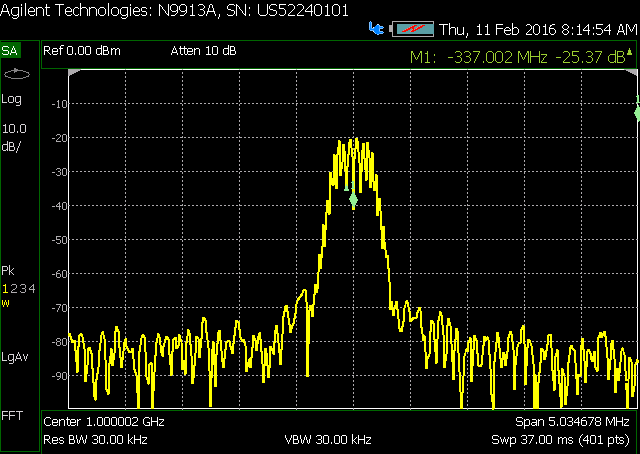
\includegraphics[width=1.0\linewidth]{tx_spec_an}
			\caption{Output of FSK App RF transmit}
			\label{fig:tx_spec_an}
		\end{minipage}
	\end{figure}
% \pagebreak
\subsection{Known Issues}
\begin{itemize}
  \item
    The input file requires pre-processing (\sref{sec:baud_sync}), so the application cannot currently transmit arbitrary user-provided files.
  \item  % AV-4043
    The demodulation algorithm currently suffers from limited carrier recovery ability which can cause the output image to be corrupted or non-existent when using the \textit{rx} or \textit{txrx} mode.
    If using an SMA loopback for txrx mode on an RF transceiver where the RX and TX data stream's LOs are sourced by the same clock, carrier recovery is not expected to be an issue.
  \item  % AV-5619 etc?
    The HDL implementations of some components treat the data as 16-bit values instead of platform-agnostic byte values.
    This results in an over-the-air transmission of the data being sent in a Little Endian manner, \textit{e.g.} the \path{0xFACE} synchronization pattern is actually \path{0xCEFA}.
    The RCC implementations default their \path{input_data_byte_grouping} parameter set to ``2'' for compatibility, but should be ``1''.
    Once the HDL implementations are redesigned to support an \path{input_data_byte_grouping} of ``1,'' all modes of the application should use it.
\end{itemize}
\newpage
\begin{appendices}
\section{Worker Parameters}
\label{app:Worker_Parameters}
\begin{minipage}[t]{.5\textwidth}
	\textbf{Common to all hardware}
	\begin{itemize}
		\item dc\_offset\_filter.hdl
			\subitem DATA\_WIDTH\_p = 16
			\subitem PEAK\_MONITOR\_p = true
		\item iq\_imbalance\_fixer.hdl
			\subitem DATA\_WIDTH\_p = 16
			\subitem ACC\_PREC\_p = 38
			\subitem PEAK\_MONITOR\_p = true
		\item complex\_mixer.hdl
			\subitem CHIPSCOPE\_p = false
			\subitem NCO\_DATA\_WIDTH\_p = 12
			\subitem INPUT\_DATA\_WIDTH\_p = 12
			\subitem CORDIC\_STAGES\_p = 16
			\subitem PEAK\_MONITOR\_p = true
		\item cic\_dec.hdl
			\subitem N = 3
			\subitem M = 1
			\subitem R = 16
			\subitem DIN\_WIDTH = 16
			\subitem ACC\_WIDTH = 28
			\subitem DOUT\_WIDTH = 16
		\item rp\_cordic.hdl
			\subitem DATA\_WIDTH = 16
			\subitem DATA\_EXT = 6
			\subitem STAGES = 16
		\item fir\_real\_sse.hdl (rx\_fir\_real)
			\subitem NUM\_TAPS\_p = 64
			\subitem DATA\_WIDTH\_p = 16
			\subitem COEFF\_WIDTH\_p = 16
		\item mfsk\_mapper.hdl
			\subitem M\_p = 2
		\item zero\_pad.hdl
			\subitem DWIDTH\_p = 16
	\end{itemize}
\end{minipage}
\begin{minipage}[t]{.5\textwidth}
	\textbf{ML605 (with FMCOMMS2/3 card in FMC HPC slot)}
	\begin{itemize}
		\item fmcomms\_2\_3\_i2c.hdl
			\subitem CP\_CLK\_FREQ\_p = 125e6
			\subitem FMC\_GA1 = 0
			\subitem FMC\_GA0 = 0
		\item ad9361\_spi.hdl
			\subitem CP\_CLK\_FREQ\_HZ\_p = 125e6
		\item ad9361\_data\_sub.hdl
			\subitem LVDS\_p = true
			\subitem DATA\_CLK\_Delay = 2
			\subitem RX\_Data\_Delay = 0
			\subitem FB\_CLK\_Delay = 7
			\subitem TX\_Data\_Delay = 0
	\end{itemize}
	\textbf{ML605 (with FMCOMMS2/3 card in FMC LPC slot)}
	\begin{itemize}
		\item fmcomms\_2\_3\_i2c.hdl
			\subitem CP\_CLK\_FREQ\_p = 125e6
			\subitem FMC\_GA1 = 1
			\subitem FMC\_GA0 = 0
		\item ad9361\_spi.hdl
			\subitem CP\_CLK\_FREQ\_HZ\_p = 125e6
		\item ad9361\_data\_sub.hdl
			\subitem LVDS\_p = true
			\subitem DATA\_CLK\_Delay = 2
			\subitem RX\_Data\_Delay = 0
			\subitem FB\_CLK\_Delay = 7
			\subitem TX\_Data\_Delay = 0
	\end{itemize}
\end{minipage}

\begin{minipage}[t]{.5\textwidth}
	\textbf{Zedboard FMCOMMS2/3 configurations)}
	\begin{itemize}
		\item fmcomms\_2\_3\_i2c.hdl
			\subitem CP\_CLK\_FREQ\_p = 100e6
			\subitem FMC\_GA1 = 0
			\subitem FMC\_GA0 = 0
		\item ad9361\_spi.hdl
			\subitem CP\_CLK\_FREQ\_HZ\_p = 100e6
		\item ad9361\_data\_sub.hdl
			\subitem LVDS\_p = true
			\subitem DATA\_CLK\_Delay = 2
			\subitem RX\_Data\_Delay = 0
			\subitem FB\_CLK\_Delay = 7
			\subitem TX\_Data\_Delay = 0
	\end{itemize}
\end{minipage}
	\begin{minipage}[t]{.5\textwidth}
		\textbf{Matchstiq-Z1 configurations}
	\begin{itemize}
		\item lime\_adc.hdl
			\subitem DRIVE\_CLK\_p = false
			\subitem USE\_CLK\_IN\_p = false
			\subitem USE\_CTL\_CLK\_p = false
			\subitem USE\_CLK\_OUT\_p = true
		\item si5338.hdl
			\subitem CLKIN\_PRESENT\_p = true
			\subitem CLKIN\_FREQ\_p = 3.072e7
			\subitem XTAL\_PRESENT\_p = false
			\subitem XTAL\_FREQ\_p = 0
			\subitem OUTPUTS\_PRESENT\_p = true, false
			\subitem INTR\_CONNECTED\_p = false
		\item matchstiq\_z1\_i2c.hdl
			\subitem NUSERS\_p = 5
			\subitem SLAVE\_ADDRESS\_p = \\0x45, 0x71, 0x48, 0x21, 0x20
			\subitem CLK\_CNT\_p = 199
	\end{itemize}
		\textbf{Zipper-related platforms (Zedboard, Stratix IV, ML605)}
	\begin{itemize}
		\item lime\_adc.hdl
			\subitem DRIVE\_CLK\_p = false
			\subitem USE\_CLK\_IN\_p = true
			\subitem USE\_CTL\_CLK\_p = false
			\subitem USE\_CLK\_OUT\_p = false
		\item si5351.hdl
			\subitem CLKIN\_PRESENT = true
			\subitem CLKIN\_FREQ = 3.072e7
			\subitem XTAL\_PRESENT = false
			\subitem XTAL\_FREQ = 0
			\subitem VC\_PRESENT = false
			\subitem OUTPUTS\_PRESENT = 0,0,1,1,1,1,0,0
			\subitem OEB\_MODE = low
			\subitem INTR\_CONNECTED = false
		\item zipper\_i2c.hdl
			\subitem NUSERS\_p = 2
	\end{itemize}
	\end{minipage}

~\pagebreak
\section{Artifacts}
\label{app:Artifacts}
\subsection{Zedboard/FMCOMMS2/3}
	\textbf{filerw (FMCOMMS2/3 not required)}
	\begin{itemize}
	\begin{minipage}[t]{.5\textwidth}
	\item fsk\_filerw\_zed\_base.bitz
	\item target-xilinx13\_3/file\_read.so
	\item target-xilinx13\_3/Baudtracking\_simple.so
	\end{minipage}
	\begin{minipage}[t]{.5\textwidth}
	\item target-xilinx13\_3/real\_digitizer.so
	\item target-xilinx13\_3/file\_write.so
	\end{minipage}
	\end{itemize}

	\textbf{filerw\_rcc}
	\begin{itemize}
	\begin{minipage}[t]{.5\textwidth}
	\item target-xilinx13\_3/file\_read.so
	\item target-xilinx13\_3/mfsk\_mapper.so
	\item target-1-xilinx13\_3/zero\_pad.so
	\item target-xilinx13\_3/fir\_real\_sse\_for\_fskapp.so
	\item target-1-xilinx13\_3/phase\_to\_amp\_cordic.so
	\end{minipage}
	\begin{minipage}[t]{.5\textwidth}
	\item target-xilinx13\_3/rp\_cordic\_for\_fskapp.so
	\item target-xilinx13\_3/fir\_real\_sse\_for\_fskapp.so
	\item target-xilinx13\_3/Baudtracking\_simple.so
	\item target-xilinx13\_3/real\_digitizer.so
	\item target-xilinx13\_3/file\_write.so
	\end{minipage}
	\end{itemize}

	\textbf{rx}
	\begin{itemize}
  \item dc\_offset\_iq\_imbalance\_mixer\_cic\_dec\_timestamper\_zed\_cfg\_1rx\_0\\
tx\_fmcomms\_2\_3\_lpc\_lvds\_cnt\_1rx\_0tx\_thruasm\_fmcomms\_2\_3\_lpc\_LVDS\_zed.bitz \\
	\begin{minipage}[t]{.5\textwidth}
	\item target-xilinx13\_3/Baudtracking\_simple.so
	\item target-xilinx13\_3/real\_digitizer.so
	\item target-xilinx13\_3/file\_write.so
	\end{minipage}
	\begin{minipage}[t]{.5\textwidth}
	\item target-xilinx13\_3/ad9361\_config\_proxy.so
	\item target-xilinx13\_3/fmcomms\_2\_3\_rx.so
	\end{minipage}
	\end{itemize}

	\textbf{tx}
	\begin{itemize}
  \item mfsk2\_zp16\_fir\_real\_phase\_to\_amp\_cordic\_cic\_int\_zed\_cfg\_0rx\_\\
1tx\_fmcomms\_2\_3\_lpc\_lvds\_cnt\_0rx\_1tx\_thruasm\_fmcomms\_2\_3\_lpc\_LVDS\_zed.bitz
\\ \\
	\begin{minipage}[t]{.5\textwidth}
	\item target-xilinx13\_3/file\_read.so
	\item target-xilinx13\_3/zipper\_tx.so
	\end{minipage}
	\begin{minipage}[t]{.5\textwidth}
	\item target-xilinx13\_3/ad9361\_config\_proxy.so
	\item target-xilinx13\_3/fmcomms\_2\_3\_tx.so
	\end{minipage}
	\end{itemize}

	\textbf{txrx} % bbloopback is not supported on FMCOMMS2/3
	\begin{itemize}
  \item fsk\_modem\_zed\_cfg\_1rx\_1tx\_fmcomms\_2\_3\_lpc\_lvds\_cnt\_1rx\_1tx\_\\
thruasm\_fmcomms\_2\_3\_lpc\_LVDS\_zed.bitz \\
	\begin{minipage}[t]{.5\textwidth}
	\item target-xilinx13\_3/file\_read.so
	\item target-xilinx13\_3/Baudtracking\_simple.so
	\item target-xilinx13\_3/real\_digitizer.so
	\item target-xilinx13\_3/file\_write.so
	\end{minipage}
	\begin{minipage}[t]{.5\textwidth}
	\item target-xilinx13\_3/ad9361\_config\_proxy.so
	\item target-xilinx13\_3/fmcomms\_2\_3\_rx.so
	\item target-xilinx13\_3/fmcomms\_2\_3\_tx.so
	\end{minipage}
	\end{itemize}

\pagebreak
\subsection{Matchstiq-Z1}
	\textbf{filerw}
	\begin{itemize}
	\begin{minipage}[t]{.5\textwidth}
	\item fsk\_filerw\_matchstiq\_z1\_base.bitz
	\item target-xilinx13\_3/file\_read.so
	\item target-xilinx13\_3/Baudtracking\_simple.so
	\end{minipage}
	\begin{minipage}[t]{.5\textwidth}
	\item target-xilinx13\_3/real\_digitizer.so
	\item target-xilinx13\_3/file\_write.so
	\end{minipage}
	\end{itemize}

	\textbf{filerw\_rcc}
	\begin{itemize}
	\begin{minipage}[t]{.5\textwidth}
	\item target-xilinx13\_3/file\_read.so
	\item target-xilinx13\_3/mfsk\_mapper.so
	\item target-1-xilinx13\_3/zero\_pad.so
	\item target-xilinx13\_3/fir\_real\_sse\_for\_fskapp.so
	\item target-1-xilinx13\_3/phase\_to\_amp\_cordic.so
	\end{minipage}
	\begin{minipage}[t]{.5\textwidth}
	\item target-xilinx13\_3/rp\_cordic\_for\_fskapp.so
	\item target-xilinx13\_3/fir\_real\_sse\_for\_fskapp.so
	\item target-xilinx13\_3/Baudtracking\_simple.so
	\item target-xilinx13\_3/real\_digitizer.so
	\item target-xilinx13\_3/file\_write.so
	\end{minipage}
	\end{itemize}

	\textbf{rx}
	\begin{itemize}
	\item dc\_offset\_iq\_imbalance\_mixer\_cic\_dec\_rp\_cordic\_fir\_real\_matchstiq\_z1\_matchstiq\_z1\_rx\_cnt\_1rx\_0tx\_ \\ thruasm\_matchstiq\_z1.bitz \\ \\
	\begin{minipage}[t]{.5\textwidth}\item target-xilinx13\_3/Baudtracking\_simple.so
	\item target-xilinx13\_3/real\_digitizer.so
	\item target-xilinx13\_3/file\_write.so
	\item target-xilinx13\_3/matchstiq\_z1\_rx.so
	\item target-xilinx13\_3/lime\_rx\_proxy.so
	\end{minipage}
	\begin{minipage}[t]{.5\textwidth}	\item target-xilinx13\_3/si5338\_proxy.so
	\item target-xilinx13\_3/matchstiq\_z1\_avr\_proxy.so
	\item target-xilinx13\_3/tmp100\_proxy.so
	\item target-xilinx13\_3/matchstiq\_z1\_pca9535\_proxy.so
	\end{minipage}
	\end{itemize}

	\textbf{tx}
	\begin{itemize}
	\item
mfsk2\_zp16\_fir\_real\_phase\_to\_amp\_cordic\_cic\_int\_matchstiq\_z1\_matchstiq\_z1\_tx\_cnt\_0rx\_1tx\_thruasm\_matchstiq\_z1.bitz	\\ \\
	\begin{minipage}[t]{.5\textwidth}
	\item target-xilinx13\_3/file\_read.so
	\item target-xilinx13\_3/matchstiq\_z1\_tx.so
	\item target-xilinx13\_3/lime\_tx\_proxy.so
	\item target-xilinx13\_3/si5338\_proxy.so
	\end{minipage}
	\begin{minipage}[t]{.5\textwidth}
	\item target-xilinx13\_3/matchstiq\_z1\_avr\_proxy.so
	\item target-xilinx13\_3/tmp100\_proxy.so
	\item target-xilinx13\_3/matchstiq\_z1\_pca9535\_proxy.so
	\end{minipage}
	\end{itemize}

	\textbf{txrx/bbloopback}
	\begin{itemize}
	\item fsk\_modem\_matchstiq\_z1\_matchstiq\_z1\_rx\_tx\_cnt\_1rx\_1tx\_thruasm\_matchstiq\_z1.bitz \\ \\
	\begin{minipage}[t]{.5\textwidth}
	\item target-xilinx13\_3/file\_read.so
	\item target-xilinx13\_3/Baudtracking\_simple.so
	\item target-xilinx13\_3/real\_digitizer.so
	\item target-xilinx13\_3/file\_write.so
	\item target-xilinx13\_3/matchstiq\_z1\_rx.so
	\item target-xilinx13\_3/matchstiq\_z1\_tx.so
	\end{minipage}
	\begin{minipage}[t]{.5\textwidth}
	\item target-xilinx13\_3/lime\_rx\_proxy.so
	\item target-xilinx13\_3/lime\_tx\_proxy.so
	\item target-xilinx13\_3/si5338\_proxy.so
	\item target-xilinx13\_3/matchstiq\_z1\_avr\_proxy.so
	\item target-xilinx13\_3/tmp100\_proxy.so
	\item target-xilinx13\_3/matchstiq\_z1\_pca9535\_proxy.so
	\end{minipage}
	\end{itemize}

\pagebreak
\subsection{ML605/FMCOMMS2/3}
	\textbf{filerw (FMCOMMS2/3 not required)}
	\begin{itemize}
	\begin{minipage}[t]{.5\textwidth}
	\item fsk\_filerw\_ml605\_base.bitz
	\item target-centos7/file\_read.so
	\item target-centos7/Baudtracking\_simple.so
	\end{minipage}
	\begin{minipage}[t]{.5\textwidth}
	\item target-centos7/real\_digitizer.so
	\item target-centos7/file\_write.so
	\end{minipage}
	\end{itemize}

	\textbf{rx}
	\begin{itemize}
	\begin{minipage}[t]{.5\textwidth}
	\item target-centos7/file\_read.so
	\item target-centos7/Baudtracking\_simple.so
	\item target-centos7/real\_digitizer.so
	\end{minipage}
	\begin{minipage}[t]{.5\textwidth}
	\item target-centos7/ad9361\_config\_proxy.so
	\item target-centos7/fmcomms\_2\_3\_rx.so
	\end{minipage}
	\end{itemize}
	For FMCOMMS2/3 plugged into FMC LPC:
	\begin{itemize}
	\item dc\_offset\_iq\_imbalance\_mixer\_cic\_dec\_timestamper\_ml605\_cfg\_1rx\_0tx \\
\_fmcomms\_2\_3\_lpc\_lvds\_cnt\_1rx\_0tx\_thruasm\_fmcomms\_2\_3\_lpc\_LVDS\_ml605.bitz
	\end{itemize}
	For FMCOMMS2/3 plugged into FMC HPC:
	\begin{itemize}
	\item dc\_offset\_iq\_imbalance\_mixer\_cic\_dec\_timestamper\_ml605\_cfg\_1rx\_0tx \\
\_fmcomms\_2\_3\_hpc\_lvds\_cnt\_1rx\_0tx\_thruasm\_fmcomms\_2\_3\_hpc\_LVDS\_ml605.bitz
	\end{itemize}

	\textbf{tx}
	\begin{itemize}
	\begin{minipage}[t]{.5\textwidth}
	\item target-centos7/file\_read.so
	\end{minipage}
	\begin{minipage}[t]{.5\textwidth}
	\item target-centos7/ad9361\_config\_proxy.so
	\item target-centos7/fmcomms\_2\_3\_tx.so
	\end{minipage}
	\end{itemize}

	\textbf{txrx} % bbloopback is not supported on FMCOMMS2/3
	\begin{itemize}
	\begin{minipage}[t]{.5\textwidth}
	\item target-centos7/file\_read.so
	\item target-centos7/Baudtracking\_simple.so
	\item target-centos7/real\_digitizer.so
	\end{minipage}
	\begin{minipage}[t]{.5\textwidth}
	\item target-centos7/ad9361\_config\_proxy.so
	\item target-centos7/fmcomms\_2\_3\_rx.so
	\item target-centos7/fmcomms\_2\_3\_tx.so
	\end{minipage}
	\end{itemize}

\pagebreak
\subsection{Host-only CentOS 7}
	\textbf{filerw\_rcc}
	\begin{itemize}
	\begin{minipage}[t]{.5\textwidth}
	\item target-centos7/file\_read.so
	\item target-centos7/mfsk\_mapper.so
	\item target-1-centos7/zero\_pad.so
	\item target-centos7/fir\_real\_sse\_for\_fskapp.so
	\item target-1-centos7/phase\_to\_amp\_cordic.so
	\end{minipage}
	\begin{minipage}[t]{.5\textwidth}
	\item target-centos7/rp\_cordic\_for\_fskapp.so
	\item target-centos7/fir\_real\_sse\_for\_fskapp.so
	\item target-centos7/Baudtracking\_simple.so
	\item target-centos7/real\_digitizer.so
	\item target-centos7/file\_write.so
	\end{minipage}
	\end{itemize}

\pagebreak
\section{Deprecated Zipper}
\label{app:Zipper}
Beginning with OpenCPI Version 1.5, Support for Lime Microsystems' Zipper card is now deprecated, and the following have been removed from the main body of this document:\medskip

\subsection{Supported Hardware Setups}
This app is supported on the following hardware configurations:
\begin{itemize}
  \item Zedboard/Zipper/MyriadRF
  \item x86/Stratix IV GX development kit (230 Edition)/Zipper/MyriadRF in HSMC A slot
  \item x86/Stratix IV GX development kit (230 Edition)/Zipper/MyriadRF in HSMC B slot
  \item x86/ML605/Zipper/MyriadRF in FMC LPC slot
  \item x86/ML605/Zipper/MyriadRF in FMC HPC slot
\end{itemize}

\subsection{Known Issues}
\begin{itemize}
  \item For more information on known limitations when using the Zipper-related platforms (Zedboard, Stratix IV, ML605), see the document Myriad-RF\_1\_Zipper\_Limitations included with this project.
  \item  On x86 host machines with more than one Stratix IV and/or ML605s plugged into PCIe slots, this app will assume that the first found Stratix IV/ML605 has a Zipper/MyriadRF plugged in. The first found Stratix IV/ML605 will be used during execution. While there are means to address this issue, they have not been implemented for the current release.
\end{itemize}

\subsection{Additional Dependencies for Zipper-related platforms (Zedboard, Stratix IV, ML605)}
	\begin{tabular}{|c|c|c|c|c|c|}
	\hline
	\rowcolor{blue}
	Application XML & filerw & rx & tx & txrx & bbloopback \\
	\hline
	\checkrow{app\_fsk\_rx\_zipper (dependency only, no build required)}{ }{x}{ }{ }{ }
	\hline
	\checkrow{app\_fsk\_tx\_zipper (dependency only, no build required)}{ }{ }{x}{ }{ }
	\hline
	\checkrow{app\_fsk\_txrx\_zipper (dependency only, no build required)}{ }{ }{ }{x}{x}
	\hline
	\rowcolor{blue}
	RX Path Workers & filerw & rx & tx & txrx & bbloopback \\
	\hline
	\checkrow{lime\_adc.hdl}{ }{x}{ }{x}{x}
	\hline
	\rowcolor{blue}
	TX Path Workers & filerw & rx & tx & txrx & bbloopback \\
	\hline
	\checkrow{lime\_dac.hdl}{ }{ }{x}{x}{x}
	\hline
	\rowcolor{blue}
	Endpoint Proxies & filerw & rx & tx & txrx & bbloopback \\
	\hline
	\checkrow{zipper\_rx.rcc}{ }{x}{ }{x}{x}
	\hline
	\checkrow{zipper\_tx.rcc}{ }{ }{x}{x}{x}
	\hline
	\rowcolor{blue}
	SPI Command and Control & filerw & rx & tx & txrx & bbloopback \\
	\hline
	\checkrow{lime\_rx\_proxy.rcc}{ }{x}{ }{x}{x}
	\hline
	\checkrow{lime\_rx.hdl}{ }{x}{ }{x}{x}
	\hline
	\checkrow{lime\_tx\_proxy.rcc}{ }{ }{x}{x}{x}
	\hline
	\checkrow{lime\_tx.hdl}{ }{ }{x}{x}{x}
	\hline
	\checkrow{lime\_spi.hdl}{ }{x}{x}{x}{x}
	\hline
	\rowcolor{blue}
	I2C Command and Control & filerw & rx & tx & txrx & bbloopback \\
	\hline
	\checkrow{si5351\_proxy.rcc}{ }{x}{x}{x}{x}
	\hline
	\checkrow{si5351.hdl}{ }{x}{x}{x}{x}
	\hline
	\end{tabular}

\medskip

\subsection{Zipper Recommended Library Path}
\textbf{Recommended Library Path for Stratix IV GX230/Zipper in HSMC A}\\

\textbf{\textit{rx}}\\
\verb|OCPI_LIBRARY_PATH=../../artifacts/ocpi.assets.dc_offset_iq_imbalance_mixer_cic_dec_\| \\
\verb|rp_cordic_fir_real_alst4_alst4_zipper_hsmc_alst4_port_a_rx_cnt_1rx_0tx_thruasm_zipper_\| \\
\verb|hsmc_a_alst4.hdl.0.alst4.gz\| \\
\verb|:../../core/artifacts:../../artifacts| \\

\textbf{\textit{tx}}\\
\verb|OCPI_LIBRARY_PATH=../../artifacts/ocpi.assets.mfsk2_zp16_fir_real_phase_to_amp_cordic_cic_int_\| \\
\verb|alst4_alst4_zipper_hsmc_alst4_port_a_tx_cnt_0rx_1tx_thruasm_zipper_hsmc_a_alst4.hdl.0.alst4.gz\| \\
\verb|:../../core/artifacts:../../artifacts| \\

\textbf{\textit{txrx/bbloopback}}\\
\verb|OCPI_LIBRARY_PATH=../../artifacts/ocpi.assets.fsk_modem_alst4_alst4_zipper_hsmc_alst4_\| \\
\verb|port_a_rx_tx_cnt_1rx_1tx_thruasm_zipper_hsmc_a_alst4.hdl.0.alst4.gz\| \\
\verb|:../../core/artifacts:../../artifacts| \\
\par\medskip

\textbf{Recommended Library Path for Stratix IV GX230/Zipper in HSMC B}\\

\textbf{\textit{rx}}\\
\verb|OCPI_LIBRARY_PATH=../../artifacts/ocpi.assets.dc_offset_iq_imbalance_mixer_cic_dec_rp_cordic_fir\| \\
\verb|_real_alst4_alst4_zipper_hsmc_alst4_port_b_rx_cnt_1rx_0tx_thruasm_zipper_hsmc_b_alst4.hdl.0.alst4.gz\| \\
\verb|:../../../core/artifacts:../../artifacts| \\

\textbf{\textit{tx}}\\
\verb|OCPI_LIBRARY_PATH=../../artifacts/ocpi.assets.mfsk2_zp16_fir_real_phase_to_amp_cordic_cic_int\| \\
\verb|_alst4_alst4_zipper_hsmc_alst4_port_b_tx_cnt_0rx_1tx_thruasm_zipper_hsmc_b_alst4.hdl.0.alst4.gz\| \\
\verb|:../../../core/artifacts:../../artifacts| \\

\textbf{\textit{txrx/bbloopback}}\\
\verb|OCPI_LIBRARY_PATH=../../artifacts/ocpi.assets.fsk_modem_alst4_alst4_zipper_hsmc_alst4_\| \\
\verb|port_b_rx_tx_cnt_1rx_1tx_thruasm_zipper_hsmc_b_alst4.hdl.0.alst4.gz\| \\
\verb|:../../../core/artifacts:../../artifacts| \\
\par\medskip


\textbf{Recommended Library Path for ML605/Zipper in FMC LPC}\\

\textbf{\textit{rx}}\\
\verb|OCPI_LIBRARY_PATH=../../artifacts/ocpi.assets.dc_offset_iq_imbalance_mixer_cic_dec_rp_cordic\| \\
\verb|_fir_real_ml605_ml605_zipper_fmc_lpc_rx_cnt_1rx_0tx_thruasm_zipper_lpc_ml605.hdl.0.ml605.gz\| \\
\verb|:../../../core/artifacts:../../artifacts| \\

\textbf{\textit{tx}}\\
\verb|OCPI_LIBRARY_PATH=../../artifacts/ocpi.assets.fsk_modem_ml605_ml605\| \\
\verb|_zipper_fmc_lpc_rx_tx_cnt_1rx_1tx_thruasm_zipper_lpc_ml605.hdl.0.ml605.gz\| \\
\verb|:../../../core/artifacts:../../artifacts| \\

\textbf{\textit{txrx/bbloopback}}\\
\verb|OCPI_LIBRARY_PATH=../../artifacts/ocpi.assets.fsk_modem_ml605_ml605\| \\
\verb|_zipper_fmc_lpc_rx_tx_cnt_1rx_1tx_thruasm_zipper_lpc_ml605.hdl.0.ml605.gz\| \\
\verb|:../../../core/artifacts:../../artifacts| \\
\par\medskip

\textbf{Example ML605/Zipper in FMC HPC}\\
\textbf{\textit{rx}}\\
\verb|OCPI_LIBRARY_PATH=../../artifacts/ocpi.assets.dc_offset_iq_imbalance_mixer_cic_dec_rp_cordic\| \\
\verb|_fir_real_ml605_ml605_zipper_fmc_hpc_rx_cnt_1rx_0tx_thruasm_zipper_hpc_ml605.hdl.0.ml605.gz\| \\
\verb|:../../../core/artifacts:../../artifacts| \\

\textbf{\textit{tx}}\\
\verb|OCPI_LIBRARY_PATH=../../artifacts/ocpi.assets.mfsk2_zp16_fir_real_phase_to_amp_cordic_cic_int\| \\
\verb|_ml605_ml605_zipper_fmc_hpc_tx_cnt_0rx_1tx_thruasm_zipper_hpc_ml605.hdl.0.ml605.gz\| \\
\verb|:../../../core/artifacts:../../artifacts| \\

\textbf{\textit{txrx/bbloopback}}\\
\verb|OCPI_LIBRARY_PATH=../../artifacts/ocpi.assets.fsk_modem_ml605_ml605\| \\
\verb|_zipper_fmc_hpc_rx_tx_cnt_1rx_1tx_thruasm_zipper_hpc_ml605.hdl.0.ml605.gz\| \\
\verb|:../../../core/artifacts:../../artifacts| \\


\pagebreak

\subsection{Artifacts: Zedboard/Zipper}
	\textbf{filerw (zipper not required)}
	\begin{itemize}
	\begin{minipage}[t]{.5\textwidth}
	\item fsk\_filerw\_zed\_base.bitz
	\item target-xilinx13\_3/file\_read.so
	\item target-xilinx13\_3/Baudtracking\_simple.so
	\end{minipage}
	\begin{minipage}[t]{.5\textwidth}
	\item target-xilinx13\_3/real\_digitizer.so
	\item target-xilinx13\_3/file\_write.so
	\end{minipage}
	\end{itemize}

	\textbf{rx}
	\begin{itemize}
	\item dc\_offset\_iq\_imbalance\_mixer\_cic\_dec\_rp\_cordic\_fir\_real\_zed\_base\_cnt\_1rx\_0tx\_thruasm\_zipper\_lpc\_zed.bitz \\ \\
	\begin{minipage}[t]{.5\textwidth}
	\item target-xilinx13\_3/Baudtracking\_simple.so
	\item target-xilinx13\_3/real\_digitizer.so
	\item target-xilinx13\_3/file\_write.so
	\end{minipage}
	\begin{minipage}[t]{.5\textwidth}
	\item target-xilinx13\_3/zipper\_rx.so
	\item target-xilinx13\_3/lime\_rx\_proxy.so
	\item target-xilinx13\_3/si5351\_proxy.so
	\end{minipage}
	\end{itemize}

	\textbf{tx}
	\begin{itemize}
	\item mfsk2\_zp16\_fir\_real\_phase\_to\_amp\_cordic\_cic\_int\_zed\_base\_cnt\_0rx\_1tx\_thruasm\_zipper\_lpc\_zed.bitz
\\ \\
	\begin{minipage}[t]{.5\textwidth}
	\item target-xilinx13\_3/file\_read.so
	\item target-xilinx13\_3/zipper\_tx.so
	\end{minipage}
	\begin{minipage}[t]{.5\textwidth}
	\item target-xilinx13\_3/lime\_tx\_proxy.so
	\item target-xilinx13\_3/si5351\_proxy.so
	\end{minipage}
	\end{itemize}

	\textbf{txrx/bbloopback}
	\begin{itemize}
	\item fsk\_modem\_zed\_base\_cnt\_1rx\_1tx\_thruasm\_zipper\_lpc\_zed.bitz \\ \\
	\begin{minipage}[t]{.5\textwidth}
	\item target-xilinx13\_3/file\_read.so
	\item target-xilinx13\_3/Baudtracking\_simple.so
	\item target-xilinx13\_3/real\_digitizer.so
	\item target-xilinx13\_3/file\_write.so
	\end{minipage}
	\begin{minipage}[t]{.5\textwidth}
	\item target-xilinx13\_3/zipper\_rx.so
	\item target-xilinx13\_3/zipper\_tx.so
	\item target-xilinx13\_3/lime\_rx\_proxy.so
	\item target-xilinx13\_3/lime\_tx\_proxy.so
	\item target-xilinx13\_3/si5351\_proxy.so
	\end{minipage}
	\end{itemize}

\pagebreak
\subsection{Artifacts: Stratix IV/Zipper}
	\textbf{filerw (zipper not required)}
	\begin{itemize}
	\begin{minipage}[t]{.5\textwidth}
	\item fsk\_filerw\_alst4\_base.bitz
	\item target-centos7/file\_read.so
	\item target-centos7/Baudtracking\_simple.so
	\end{minipage}
	\begin{minipage}[t]{.5\textwidth}
	\item target-centos7/real\_digitizer.so
	\item target-centos7/file\_write.so
	\end{minipage}
	\end{itemize}

	\textbf{rx}
	\begin{itemize}
	\begin{minipage}[t]{.5\textwidth}
	\item target-centos7/file\_read.so
	\item target-centos7/Baudtracking\_simple.so
	\item target-centos7/real\_digitizer.so
	\end{minipage}
	\begin{minipage}[t]{.5\textwidth}
	\item target-centos7/zipper\_rx.so
	\item target-centos7/lime\_rx\_proxy.so
	\item target-centos7/si5351\_proxy.so
	\end{minipage}
	\end{itemize}
	For Zipper plugged into HSMC Port A:
	\begin{itemize}
	\item dc\_offset\_iq\_imbalance\_mixer\_cic\_dec\_rp\_cordic\_fir\_real\_alst4\_alst4\_zipper\_hsmc\_alst4\_port\_a\_ \\
		rx\_cnt\_1rx\_0tx\_thruasm\_zipper\_hsmc\_a\_alst4.bitz
	\end{itemize}
	For Zipper plugged into HSMC Port B:
	\begin{itemize}
	\item dc\_offset\_iq\_imbalance\_mixer\_cic\_dec\_rp\_cordic\_fir\_real\_alst4\_alst4\_zipper\_hsmc\_alst4\_port\_b\_ \\
		rx\_cnt\_1rx\_0tx\_thruasm\_zipper\_hsmc\_b\_alst4.bitz
	\end{itemize}

	\textbf{tx}
	\begin{itemize}
	\begin{minipage}[t]{.5\textwidth}
	\item target-centos7/file\_read.so
	\item target-centos7/zipper\_tx.so
	\end{minipage}
	\begin{minipage}[t]{.5\textwidth}
	\item target-centos7/lime\_tx\_proxy.so
	\item target-centos7/si5351\_proxy.so
	\end{minipage}
	\end{itemize}
	For Zipper plugged into HSMC Port A:
	\begin{itemize}
	\item mfsk2\_zp16\_fir\_real\_phase\_to\_amp\_cordic\_cic\_int\_alst4\_alst4\_zipper\_hsmc\_alst4\_port\_a\_\\
		txcnt\_0rx\_1tx\_thruasm\_zipper\_hsmc\_a\_alst4.bitz
	\end{itemize}
	For Zipper plugged into HSMC Port B:
	\begin{itemize}
	\item mfsk2\_zp16\_fir\_real\_phase\_to\_amp\_cordic\_cic\_int\_alst4\_alst4\_zipper\_hsmc\_alst4\_port\_b\_\\
		tx\_cnt\_0rx\_1tx\_thruasm\_zipper\_hsmc\_b\_alst4.bitz
	\end{itemize}

	\textbf{txrx/bbloopback}
	\begin{itemize}
	\begin{minipage}[t]{.5\textwidth}
	\item target-centos7/file\_read.so
	\item target-centos7/Baudtracking\_simple.so
	\item target-centos7/real\_digitizer.so
	\item target-centos7/zipper\_rx.so
	\end{minipage}
	\begin{minipage}[t]{.5\textwidth}
	\item target-centos7/zipper\_tx.so
	\item target-centos7/lime\_rx\_proxy.so
	\item target-centos7/lime\_tx\_proxy.so
	\item target-centos7/si5351\_proxy.so
	\end{minipage}
	\end{itemize}
	For Zipper plugged into HSMC Port A:
	\begin{itemize}
		\item fsk\_modem\_alst4\_alst4\_zipper\_hsmc\_alst4\_port\_a\_rx\_tx\_cnt\_1rx\_1tx\_thruasm\_zipper\_hsmc\_a\_alst4.bitz
	\end{itemize}
	For Zipper plugged into HSMC Port B:
	\begin{itemize}
		\item fsk\_modem\_alst4\_alst4\_zipper\_hsmc\_alst4\_port\_b\_rx\_tx\_cnt\_1rx\_1tx\_thruasm\_zipper\_hsmc\_b\_alst4.bitz
	\end{itemize}

\pagebreak
\subsection{Artifacts: ML605/Zipper}
	\textbf{filerw (zipper not required)}
	\begin{itemize}
	\begin{minipage}[t]{.5\textwidth}
	\item fsk\_filerw\_ml605\_base.bitz
	\item target-centos7/file\_read.so
	\item target-centos7/Baudtracking\_simple.so
	\end{minipage}
	\begin{minipage}[t]{.5\textwidth}
	\item target-centos7/real\_digitizer.so
	\item target-centos7/file\_write.so
	\end{minipage}
	\end{itemize}

	\textbf{rx}
	\begin{itemize}
	\begin{minipage}[t]{.5\textwidth}
	\item target-centos7/file\_read.so
	\item target-centos7/Baudtracking\_simple.so
	\item target-centos7/real\_digitizer.so
	\end{minipage}
	\begin{minipage}[t]{.5\textwidth}
	\item target-centos7/zipper\_rx.so
	\item target-centos7/lime\_rx\_proxy.so
	\item target-centos7/si5351\_proxy.so
	\end{minipage}
	\end{itemize}
	For Zipper plugged into FMC LPC:
	\begin{itemize}
	\item dc\_offset\_iq\_imbalance\_mixer\_cic\_dec\_rp\_cordic\_fir\_real\_ml605\_cfg\_1rx\_0tx\_fmcomms\_2\_3\_lpc\_ \\
	lvds\_cnt\_1rx\_0tx\_thruasm\_fmcomms\_2\_3\_lpc\_LVDS\_ml605.bitz
	\end{itemize}
	For Zipper plugged into FMC HPC:
	\begin{itemize}
	\item dc\_offset\_iq\_imbalance\_mixer\_cic\_dec\_rp\_cordic\_fir\_real\_ml605\_cfg\_1rx\_0tx\_fmcomms\_2\_3\_hpc\_ \\
	lvds\_cnt\_1rx\_0tx\_thruasm\_fmcomms\_2\_3\_hpc\_LVDS\_ml605.bitz
	\end{itemize}

	\textbf{tx}
	\begin{itemize}
	\begin{minipage}[t]{.5\textwidth}
	\item target-centos7/file\_read.so
	\item target-centos7/zipper\_tx.so
	\end{minipage}
	\begin{minipage}[t]{.5\textwidth}
	\item target-centos7/lime\_tx\_proxy.so
	\item target-centos7/si5351\_proxy.so
	\end{minipage}
	\end{itemize}
	For Zipper plugged into FMC LPC:
	\begin{itemize}
		\item mfsk2\_zp16\_fir\_real\_phase\_to\_amp\_cordic\_cic\_int\_ml605\_ml605\_zipper\_fmc\_lpc\_ \\
		tx\_cnt\_0rx\_1tx\_thruasm\_zipper\_lpc\_ml605.bitz
	\end{itemize}
	For Zipper plugged into FMC HPC:
	\begin{itemize}
		\item mfsk2\_zp16\_fir\_real\_phase\_to\_amp\_cordic\_cic\_int\_ml605\_ml605\_zipper\_fmc\_hpc\_ \\
		tx\_cnt\_0rx\_1tx\_thruasm\_zipper\_hpc\_ml605.bitz
	\end{itemize}

	\textbf{txrx/bbloopback}
	\begin{itemize}
	\begin{minipage}[t]{.5\textwidth}
	\item target-centos7/file\_read.so
	\item target-centos7/Baudtracking\_simple.so
	\item target-centos7/real\_digitizer.so
	\item target-centos7/zipper\_rx.so
	\end{minipage}
	\begin{minipage}[t]{.5\textwidth}
	\item target-centos7/zipper\_tx.so
	\item target-centos7/lime\_rx\_proxy.so
	\item target-centos7/lime\_tx\_proxy.so
	\item target-centos7/si5351\_proxy.so
	\end{minipage}
	\end{itemize}
	For Zipper plugged into FMC LPC:
	\begin{itemize}
		\item fsk\_modem\_ml605\_ml605\_zipper\_fmc\_hpc\_rx\_tx\_cnt\_1rx\_1tx\_thruasm\_zipper\_lpc\_ml605.bitz
	\end{itemize}
	For Zipper plugged into FMC HPC:
	\begin{itemize}
		\item fsk\_modem\_ml605\_ml605\_zipper\_fmc\_hpc\_rx\_tx\_cnt\_1rx\_1tx\_thruasm\_zipper\_hpc\_ml605.bitz
	\end{itemize}
\end{appendices}
\end{document}
